\documentclass[12pt,a4paper,openany]{report}
%%%% JNLP 
\usepackage{lmodern}
\usepackage{xcolor}
\usepackage[utf8]{inputenc}
\usepackage[T1]{fontenc}
\usepackage[francais]{babel}
\usepackage[top=1.7cm, bottom=1.7cm, left=1.5cm, right=1.5cm]{geometry}
\usepackage{pdfpages}
\usepackage{listingsutf8}
\usepackage{fancyhdr}
\usepackage{multido}
\usepackage{multicol}
\usepackage{amssymb}
\usepackage{tikz}
\usepackage{ifthen}
\usepackage{makeidx}
\usepackage[urlbordercolor={1 1 1}, linkbordercolor={1 1 1}, urlcolor=blue]{hyperref}

\newcommand{\headGauche}{}
\newcommand{\headCentre}{}
\newcommand{\headDroite}{}
%\newCommand{\footGauche}{} Université paul sabatier Toulouse III
\newcommand{\footCentre}{}
%\newCommand{\footDroite}{} Numéro de page
\newcommand{\premierDestinataire}{Monsieur Max Chevalier}
\newcommand{\rolePremierDestinataire}{Resonsable projet}

\newcommand{\secondDestinaire}{Madame Caroline Kross}
\newcommand{\roleSecondDestinaire}{Tutrice}

\newcommand{\troisiemeDestinaire}{Monsieur Thierry Millan}
\newcommand{\roleTroisiemeDestinaire}{Client}

\newcommand{\quatriemeDestinaire}{}
\newcommand{\roleQuatriemeDestinaire}{}

\newcommand{\cinquiemeDestinaire}{}
\newcommand{\roleCinquiereDestinaire}{}
\newcommand{\titreDocument}{Les plans et les cahiers de tests}



\date{\today}

\chead{\headCentre}
\rhead{\headDroite}
\lhead{\headGauche}
\makeindex
\lfoot{Université Paul Sabatier Toulouse III}
\rfoot{--~\thepage~--}
\cfoot{\footCentre}
\makeglossary
\makeatletter
\def\clap#1{\hbox to 0pt{\hss #1\hss}}%
\def\ligne#1{%
\hbox to \hsize{%
\vbox{\centering #1}}}%
\def\haut#1#2#3{%
\hbox to \hsize{%
\rlap{\vtop{\raggedright #1}}%
\hss
\clap{\vtop{\centering #2}}%
\hss
\llap{\vtop{\raggedleft #3}}}}%
\def\bas#1#2#3{%
\hbox to \hsize{%
\rlap{\vbox{\raggedright #1}}%
\hss \clap{\vbox{\centering #2}}%
\hss
\llap{\vbox{\raggedleft #3}}}}%
\def\maketitle{%
\thispagestyle{empty}\vbox to \vsize{%
\haut{}{\@blurb}{}
\begin{flushleft}
	\vspace{1cm}
	Antoine de \bsc{Roquemaurel}\\ 
	Mathieu \bsc{Soum}\\
	Geoffroy \bsc{Subias}\\
	Marie-Ly \bsc{Tang}\\
	\textit{Groupe B}\\
\end{flushleft}
\begin{flushright}
	\vspace{-3cm}
	\ifthenelse{\equal{\premierDestinataire}{}}{
	}
	{
		Pour \premierDestinataire(\rolePremierDestinataire)\\
	}
	\ifthenelse{\equal{\secondDestinaire}{}}{
	}
	{
		Pour \secondDestinaire(\roleSecondDestinaire)\\
	}
	\ifthenelse{\equal{\troisiemeDestinaire}{}}{
	}
	{
		Pour \troisiemeDestinaire(\roleTroisiemeDestinaire)\\
	}
	\ifthenelse{\equal{\quatriemeDestinaire}{}}{
	}
	{
		Pour \quatriemeDestinaire(\roleQuatriemeDestinaire)\\
	}
	\ifthenelse{\equal{\cinquiemeDestinaire}{}}{
	}
	{
		Pour \cinquiemeDestinaire(\roleCinquiereDestinaire)\\
	}
\end{flushright}
\vfill
\vspace{1cm}
\begin{flushleft}
\usefont{OT1}{ptm}{m}{n}
\huge \@title
\end{flushleft}
\par
\hrule height 4pt
\par
\begin{flushright}
\usefont{OT1}{phv}{m}{n}
\Large \@author
\par
\end{flushright}
\vspace{1cm}
\vfill
\vfill
\bas{}{\@location, le \@date}{}
}%
\cleardoublepage
}
\def\date#1{\def\@date{#1}}
\def\author#1{\def\@author{#1}}
\def\title#1{\def\@title{#1}}
\def\location#1{\def\@location{#1}}
\def\blurb#1{\def\@blurb{#1}}
\date{\today}
\author{}
\title{}
\location{Amiens}\blurb{}
\makeatother
\title{\titreDocument}
\author{Bibliothèque d'objets graphiques UML}

\location{Toulouse}
\blurb{%
Université Paul Sabatier -- Toulouse III\\
IUT A - Toulouse Rangueil\\
\textbf{Projet tuteuré}\\[1em]
}%



\pagestyle{fancy}

\begin{document}
	\maketitle
	\newpage
	\setcounter{tocdepth}{4}
	\setcounter{secnumdepth}{3}
	\tableofcontents
	\newpage
	\chapter{Les plans de tests}
	\section{Les plans de non régression}
	Notre projet est de développé une bibliothèque UML\footnote{Unified Modeling Language}, aucun système n'existant
	au départ, il est donc inutile de faire un test de non régression étant donné que nous ne continuons pas un système, il n'y aura pas 
	de régression.
	\section{Les tests de validation}
		Nous avons développé un démonstrateur qui utilise notre bibliothèque et qui fait office de test de validation. Il nous permet de vérifier que toutes les attentes du client sont respectés. \\
		Avec ce démonstrateur, nous pouvons montrer au client les différentes possibilités de la bibliothèque, ainsi qu'un exemple d'utilisation.

		\subsection{Jeux d'essais}
		\subsubsection{Dessiner un diagramme complet}
		Nous avons effectués plusieurs jeux d'essais, le but est de pouvoir dessiner un pour chacun des types de diagrammes demandés par le client,
		un diagramme utilisant tous les composant de la norme UML 2.0 et respectant cette même norme, ceci pour chacun des diagrammes 
		demandés par notre client. 
		\begin{itemize}
			\item Dessiner un diagramme de classe
			\item Dessiner un diagramme de séquence
			\item Dessiner un diagramme de cas d'utilisation
		\end{itemize}
	
		\subsubsection{Respecter les contraintes d'ajout d'éléments}
		Pour chacun des diagrammes, les contraintes doivent être respectés, ainsi en fonction du type de diagramme, certains éléments ne doivent pas pouvoir
		être inséré. Voici la liste des éléments autorisés en fonction du type de diagramme.
		\begin{multicols}{2}
		\paragraph{Diagramme de cas d'utilisation}
		\begin{itemize}
			\item Cas d'utilisation
			\item Acteur actif
		\end{itemize}
		\paragraph{Diagramme de classe}
		\begin{itemize}
			\item Classe
			\item Interface
		\end{itemize}
		\paragraph{Diagramme de séquence}
		\begin{itemize}
			\item Traitement
			\item Acteur actif 
			\item Acteur passif
			\item Ligne de vie 
		\end{itemize}
		\end{multicols}

		\subsubsection{Respecter les contraintes de liaisons d'éléments}
		Nous devons également respecter les contraintes de liaison entre les différents éléments. Ainsi voici la liste des liaisons possible.
		\begin{multicols}{2}
		\paragraph{Diagramme de classe}	
		\begin{itemize}
			\item Entre deux classes
				\begin{itemize}
					\item Agrégation
					\item Composition
					\item Association
					\item Spécialisation
				\end{itemize}
			\item Entre une classe et une interface
				\begin{itemize}
					\item Spécialisation
					\item Dépendance fonctionnelle 
						\\ \\
				\end{itemize}
		\end{itemize}
		\paragraph{Diagramme de cas d'utilisation}	
		\begin{itemize}
			\item Entre un acteur un cas d'utilisation
				\begin{itemize}
					\item Association
				\end{itemize}
			\item Entre deux cas d'utilisations
				\begin{itemize}
					\item Dépendance fonctionnelle
				\end{itemize}
		\end{itemize}
		\paragraph{Diagramme de séquence}
		\begin{itemize}
			\item Entre deux traitements
				\begin{itemize}
					\item Dépendance fonctionnelle
					\item Déclenchements
				\end{itemize}
		\end{itemize}
		\end{multicols}
		\subsection{Résultats obtenus}
		Nous vérifierons que les diagrammes sont bien réalisés, qu'il n'y a aucune erreur, et qu'ils correspondent aux besoins du client.\\
		Également, nous vérifierons que nous ne pouvons pas relier ou ajouter des éléments non autorisés par la norme UML 2.0.

	\section{Les tests d'intégration}
		Nous avons développé un démonstrateur qui utilise notre bibliothèque et qui fait office de test d'intégration démontrant que notre système
		est utilisable en tant que composant par un logiciel extérieur. Il nous permet également de montrer au client les possibilités de notre bibliothèque.

		\subsection{Les composants à tester}
			Notre bibliothèque d'objet graphique en tant que composant de notre démonstrateur.

			\subsection{Les jeux d'essais}
			Dessiner un diagramme de classe, un diagramme de séquence ainsi qu'un diagramme de cas d'utilisation chacun utilisant tous les objets graphiques 
			possibles. \\
			Une fois ces diagrammes dessinés, nous testerons la suppression\footnote{La suppression d'un élément devant supprimer les liens de l'élément supprimé},
			l'ajout de méthodes et d'attributs dans une classe, ainsi que la modification de données.

			\subsection{Les résultats attendus}
			Représentation graphique des différents diagrammes respectant les normes UML 2.0 avec possibilité d'ajout ou de suppression de données.
	\section{Les tests unitaires}
	Les tests unitaires servent à tester chacune des méthodes de notre bibliothèque.\\
	Nous avons utiliser JUnit pour tester toutes les méthodes de notre bibliothèque. Les tests sont validés si 
	la bibliothèque JUnit nous indique que tous les tests passent et ne posent pas de problème.
	La description des tests unitaires est disponible sous format Javadoc à l'annexe \ref{junitdoc} page \pageref{junitdoc}.
	Elle est également disponible sous format HTML à l'adresse suivante: \\
	$\rhd$ \url{http://documentation.joohoo.fr/libUML/junitTests/index.html}\\
		
	\section{Le test de charges}
		\subsection{Le jeux d'essai}
		Le test de charge permet de savoir si la création d'un grand nombre d'élément graphique ne posera pas de problème. 
		Ainsi, nous allons créer les éléments suivants dans un diagramme sans contraintes.
		\begin{itemize}
			\item 20 Classes
			\item 20 Cas d'utilisation
			\item 20 Traitements
			\item 20 Acteurs actifs
			\item 20 Acteurs passifs
			\item 20 interface 
			\item 60 liens
		\end{itemize}
		Une fois ces éléments suivants créer, nous supprimerons 40 éléments, qui devront supprimer les liens reliés aux éléments.
		\subsection{Les résultats attendus}
		Aucune exception, les éléments ont été bien créer et certains éléments ont été supprimés avec les liens.
	\chapter{Les cahiers de tests}	
	\section{Les tests de validation}
	\section{Les tests d'intégration}
	\section{Les tests unitaires}
	Après lancement des tests unitaires, ils sont tous passéss. Nous pouvons donc en conclure que les différents modules de la bibliothèque UML fonctionnent. 
	\begin{center} 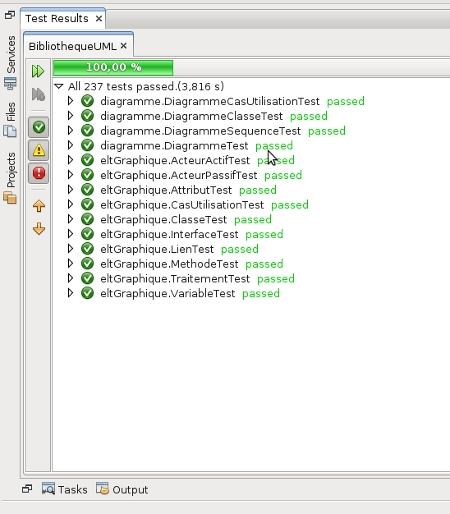
\includegraphics[width=8cm]{junitPassed.jpg} \end{center}
	\section{Le test de charge}
	\appendix	
	\chapter{Documentation des tests unitaires}
	\label{junitdoc}
	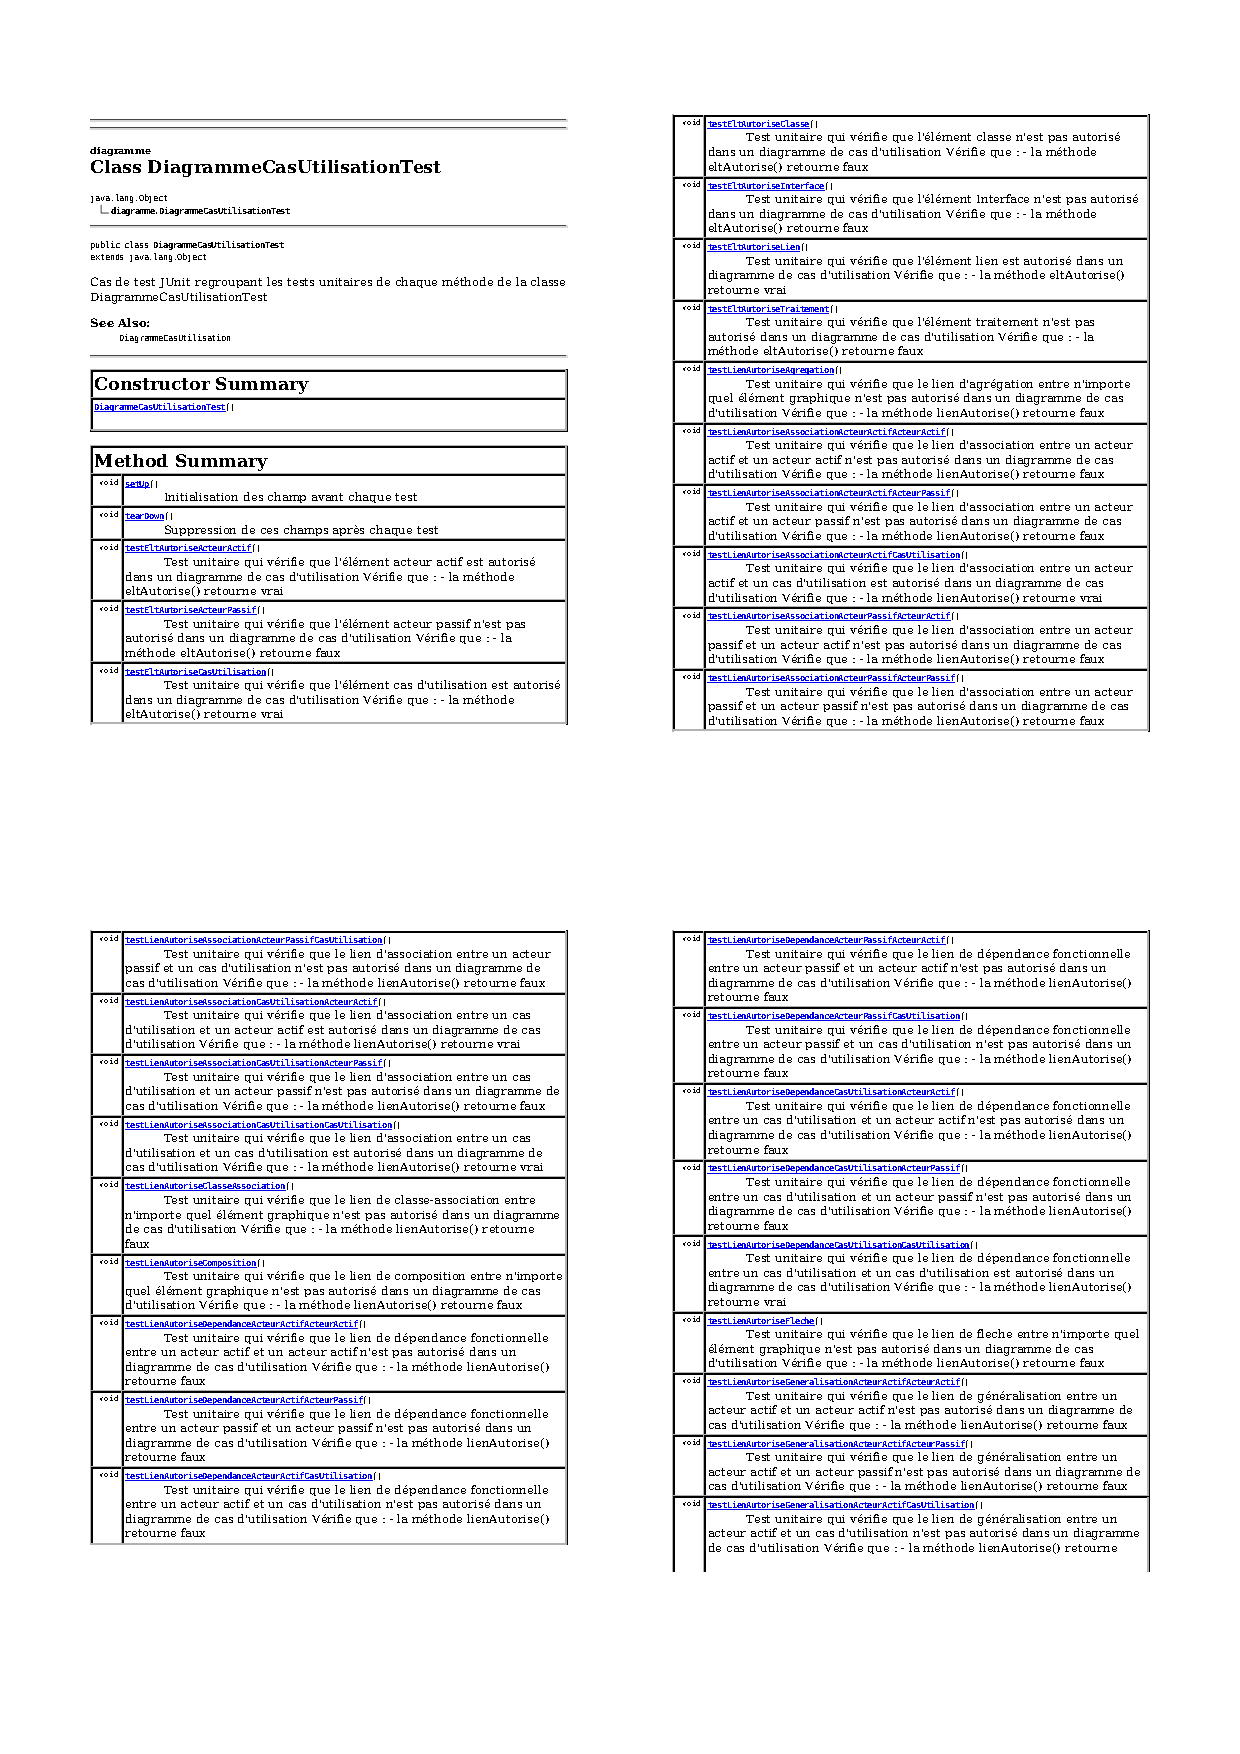
\includepdf[page=1-23]{docJUnit.pdf}
\end{document}
